\section{Results}

\begin{figure*}[t]
\centering
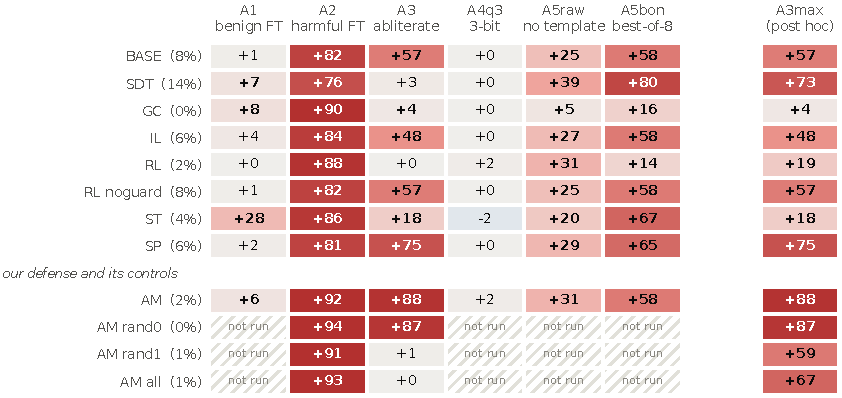
\includegraphics[width=0.92\textwidth]{figures/fig1_heatmap.pdf}
\caption{\textbf{Most fixes do not survive.} Rise in harmful-reply rate (WildGuard, percentage points) after each
post-release change, relative to the same run as released; row labels give the as-released rate. Bold: the paired
95\% bootstrap CI excludes 0 (200 prompts per cell). \att{A3max} is a post-hoc sensitivity variant of abliteration
and is never ranked. Controls of our defense ran the attacks it targets only. The same figure under Llama Guard is
in Appendix~\ref{app:tables}.}
\label{fig:heatmap}
\end{figure*}

\subsection{Do fixes survive?}
\label{sec:survive}
Figure~\ref{fig:heatmap} shows the rise in harmful replies after each change. The harmful fine-tune (\att{A2}) is
the hardest: every fix ends at \V{lg.A2.min}--\V{lg.A2.max}\% under Llama Guard (WildGuard \V{wg.A2.min}--\V{wg.A2.max}\%),
indistinguishable from the unfixed base model (\V{lg.BASE.A2}\%), while MMLU does not drop
(\run{BASE}: \V{mmlu.BASE.A0}\% before, \V{mmlu.BASE.A2}\% after; retrained and scored by log-likelihood in
Stage~2\stagetwo, \V{cap.mmlu.BASE.A0}\% and \V{cap.mmlu.BASE.A2}\%). Abliteration, with no training, takes \run{SP} from \V{wg.SP.A0}\% to
\V{wg.SP.A3}\% and \run{IL} from \V{wg.IL.A0}\% to \V{wg.IL.A3}\%; \run{GC} is the one weight-space fix that holds
(\V{wg.GC.A3}\%, also \V{wg.GC.A3max}\% at the strongest layer). The pre-registered layer rule under-attacks
\run{SDT}, which stays at \V{wg.SDT.A3}\% under \att{A3} but reaches \V{wg.SDT.A3max}\% under \att{A3max}.
Compression to 3 bits moves no run by more than \V{rise.wg.A4q3.maxabs} points (WildGuard; Llama Guard
\V{rise.lg.A4q3.maxabs}). Template removal and best-of-8 perturbations break most fixes; under \att{A5bon} only \run{GC} and the
template guard \run{RL} stay below 20\% (\V{wg.GC.A5bon}\% and \V{wg.RL.A5bon}\%), and \run{RL\_noguard} matches
\run{BASE} in every cell, so \run{RL}'s protection lives entirely in its template. A benign fine-tune leaves \run{ST}
less safe than no fix (\V{wg.ST.A1}\% vs \run{BASE} \V{wg.BASE.A1}\%).

\begin{figure}[t]
\centering
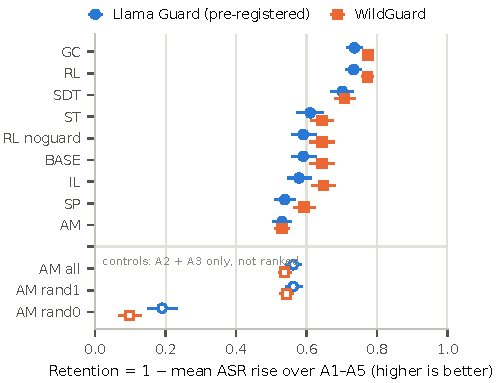
\includegraphics[width=\columnwidth]{figures/fig2_retention.pdf}
\caption{Retention with 95\% CIs (pre-registered Llama Guard judge, and WildGuard). Controls of our defense faced
only \att{A2} and \att{A3} and are not ranked.}
\label{fig:retention}
\end{figure}

\subsection{Retention ranking}
\label{sec:retention}
Under the pre-registered judge, \run{GC} ranks first (retention \V{ret.GC} \V{ret.GC.ci}) and \run{RL} second
(\V{ret.RL}); \run{BASE} scores \V{ret.BASE} and our \run{AM} ranks last (\V{ret.AM} \V{ret.AM.ci};
Fig.~\ref{fig:retention}). WildGuard gives the same top three and the same last place. Safety at release does not
predict retention: across the \V{rho.a0ret.lg.n} ranked runs, Spearman $\rho$ between as-released ASR and retention
is \V{rho.a0ret.lg} (permutation $p=\V{rho.a0ret.lg.p}$; WildGuard $\rho=\V{rho.a0ret.wg}$, $p=\V{rho.a0ret.wg.p}$). With
nine runs this is a lack of evidence for a relationship, not proof of none, but the extremes make the point: \run{AM}
is among the safest models at release (\V{wg.AM.A0}\%) and the least durable.

\begin{figure}[t]
\centering
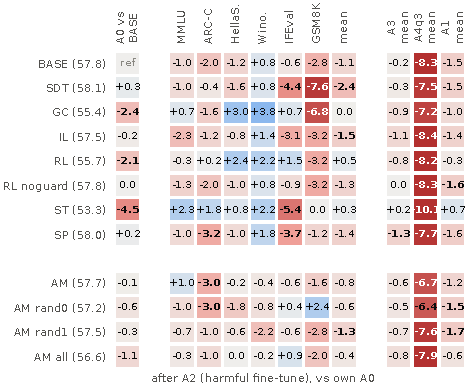
\includegraphics[width=\columnwidth]{figures/fig3_capability.pdf}
\caption{\textbf{Fixes and attacks barely move capability.} Change in accuracy (points) on six benchmarks and
their unweighted mean. Left: each fix as released vs \run{BASE}. Right: after the harmful fine-tune \att{A2} vs the
same run as released. Row labels give the as-released mean. Bold: paired 95\% bootstrap CI excludes 0 (no
multiplicity correction). Red = capability lost.}
\label{fig:capability}
\end{figure}

\subsection{Capability\stagetwo}
\label{sec:capability}
As released, \run{BASE} averages \V{cap.comp.BASE.A0}\% over the six benchmarks (MMLU \V{cap.mmlu.BASE.A0}, GSM8K
\V{cap.gsm.BASE.A0}, IFEval \V{cap.ifeval.BASE.A0}; Fig.~\ref{fig:capability}). Most fixes cost no measurable
capability. Three do: \run{ST} (\V{dcap.comp.ST.A0} points \V{dcap.comp.ST.A0.ci}; MMLU \V{dcap.mmlu.ST.A0}, GSM8K
\V{dcap.gsm.ST.A0}), \run{GC} (\V{dcap.comp.GC.A0}) and \run{RL} (\V{dcap.comp.RL.A0}). \run{RL}'s weights are
\run{BASE}'s, so its cost is the guard template (IFEval \V{dcap.ifeval.RL.A0}); \run{RL\_noguard} reproduces
\run{BASE} item for item, which also confirms that generation is deterministic. The harmful fine-tune, which removes
every fix's safety (\S\ref{sec:survive}), costs the attacker almost nothing: the mean moves by \V{dcap.comp.A2.min} to
\V{dcap.comp.A2.max} points, and the CI excludes 0 for \V{dcap.comp.A2.nsig} of \V{dcap.comp.A2.n} runs, the largest
being \run{SDT} (\V{dcap.comp.SDT.A2}, mostly GSM8K \V{dcap.gsm.SDT.A2}). No cell comes near the 30\% ``safe because
broken'' flag (lowest MMLU: \V{cap.mmlu.min}\%, \V{cap.mmlu.min.cell}). Attacked models are unsafe, not broken.
Per-benchmark scores are in Appendix~\ref{app:tables}.
\todo{add A3, A4q3 and A1 mean columns when those cells land; confirm the A2 claim with the judged Stage 2 A2 ASR.}

\subsection{Can we trust the judge?}
\label{sec:judges}
\begin{figure}[t]
\centering
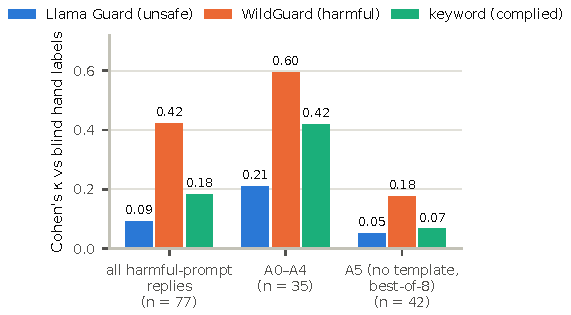
\includegraphics[width=\columnwidth]{figures/fig4_judges.pdf}
\caption{Agreement of each judge with \V{hum.nlabels} blind hand labels on harmful-prompt replies (whether the reply
gives harmful help). Both judges fall to near chance on template-stripped and perturbed text (\att{A5}).}
\label{fig:judges}
\end{figure}
Against the blind hand labels, WildGuard agrees with a human at $\kappa=\V{kappa.wg.all}$ and Llama Guard at
$\kappa=\V{kappa.lg.all}$ (Fig.~\ref{fig:judges}). On \att{A5} outputs both are near chance
($\kappa=\V{kappa.wg.afive}$ and \V{kappa.lg.afive}): Llama Guard flags \V{hum.rate.lg.afive}\% of sampled \att{A5}
replies as unsafe where the human finds \V{hum.humanrate.lg.afive}\%, mostly refusals in garbled text. Because the
judges disagree there, the headline best-of-8 number for \run{BASE} is \V{wg.BASE.A5bon}\% under WildGuard but
\V{lg.BASE.A5bon}\% under Llama Guard. We therefore report WildGuard first wherever the two judges differ by more than
10 points (a post-hoc reporting rule; rankings and tests still use the pre-registered judge). The ranking's top and
bottom do not depend on the judge (Fig.~\ref{fig:retention}).

\subsection{Our defense, and why it is a negative result}
\label{sec:defense}
\run{AM} hardens the $k=\V{cfg.am.k}$ layers whose refusal direction best separates harmful from benign dev prompts
(layers \V{cfg.am.layers}) with SafeGrad-style gradient surgery restricted to those layers, trains half of its refusal
batches with the top refusal direction ablated, and keeps those layers at \V{cfg.am.shieldbits} bits under compression.
Every choice was made on dev prompts; the recipe was frozen before its test run. \run{AM} is safer than \run{BASE} as
released under both judges (\V{lg.AM.A0}\% vs \V{lg.BASE.A0}\% Llama Guard; \V{wg.AM.A0}\% vs \V{wg.BASE.A0}\%
WildGuard) with unchanged over-refusal (\V{or.AM.A0}\% vs \V{or.BASE.A0}\%) and MMLU (\V{mmlu.AM.A0}\% vs
\V{mmlu.BASE.A0}\%). But it is \emph{worse} under abliteration (WildGuard \V{wg.AM.A3}\% vs \V{wg.BASE.A3}\%; Llama
Guard \V{lg.AM.A3}\% vs \V{lg.BASE.A3}\%), no better under the harmful fine-tune, and its located layers give no
advantage over random ones: \run{AM\_rand1} and \run{AM\_all} stay at \V{wg.AM_rand1.A3}\% and \V{wg.AM_all.A3}\%
under \att{A3}, \run{AM\_rand0} fails like \run{AM}. One plausible cause is that \run{AM}'s spread-refusal step
ablated an early-layer direction that turned out not to mediate refusal, while concentrating safety in early layers
made the model easier to abliterate. We report this as an informative negative result: locating refusal is not the
same as protecting it.
\todo{optional fig5 scatter (BASE, GC, AM, controls) once E1 composite capability lands.}

\subsection{Can we audit safety in other languages?\stagetwo}
\label{sec:multilingual}
\begin{figure}[t]
\centering
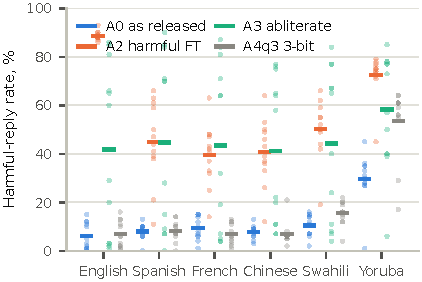
\includegraphics[width=\columnwidth]{figures/fig6_multilingual.pdf}
\caption{\textbf{Judged harmful-reply rate by language} (WildGuard on NLLB back-translations; incoherent replies count
as not harmful): bar = mean over the 12 runs, dots = single runs; 100 harmful prompts per cell, the same items in
every language. A native speaker confirms few of the Yoruba verdicts (\S\ref{sec:multilingual}), so the Yoruba bars
overstate harm.}
\label{fig:multilingual}
\end{figure}
Through the standard pipeline, translate the prompt, back-translate the reply, judge it in English, Yoruba looks far
less safe than every other language (Fig.~\ref{fig:multilingual}). As released, the judges flag
\V{mlmean.A0.yo.wg}\% of Yoruba replies against \V{mlmean.A0.en.wg}\% in English (paired gap \V{mlgap.A0.wg}
\V{mlgap.A0.wg.ci}, positive for all \V{mlgap.A0.wg.cells} runs, Llama Guard \V{mlgap.A0.lg}), and
\V{mlgap.A0.wg.rest} points more than the mean of Spanish, French, Chinese and Swahili. At 3 bits the contrast is
starkest: \V{mlmean.A4q3.yo.wg}\% vs \V{mlmean.A4q3.en.wg}\%, and for \V{mlex.nruns} models (\V{mlex.runs}) English
stays at or below \V{mlex.enmax}\% while Yoruba is judged at \V{mlex.yomin}--\V{mlex.yomax}\%. Read at face value,
an English-only audit would pass these models.

\emph{A native speaker's blind check does not support that reading.} Of 20 Yoruba replies the judges flagged
(10 as released, 10 at 3 bits), only \V{humjudge.flag.yes} actually help with the harmful request
(\V{humjudge.flag.yes.pct}\%, 95\% CI \V{humjudge.flag.yes.ci}), \V{humjudge.flag.partly} help partly and
\V{humjudge.flag.no} do not; the share is the same at both attacks (\V{humjudge.flag.A0.yes} and
\V{humjudge.flag.A4q3.yes} of 10). The judges also miss harm: \V{humjudge.ctrl.any} of \V{humjudge.ctrl.n} replies
they passed help at least partly, both at 3 bits. The translation check locates the problem in the replies, not the
prompts: \V{humyo.prompt.adequate}\% of machine-translated prompts keep their meaning (\V{humyo.prompt.harmful.adequate}\%
of harmful ones), but back-translation keeps the meaning of only \V{humyo.reply.adequate}\% of the model's Yoruba
replies, and only \V{humyo.reply.fluent}\% read as natural Yoruba. The judges are reading noisy translations of often
unnatural text, which also fits Yoruba's high over-refusal (\V{mlmean.A0.yo.or}\% vs \V{mlmean.A0.en.or}\%).
Scaling the judged rates by the confirmed share gives roughly \V{humadj.A0.yo.lo}--\V{humadj.A0.yo.hi}\% as released,
close to English, and \V{humadj.A4q3.yo.lo}--\V{humadj.A4q3.yo.hi}\% at 3 bits, perhaps above English's
\V{mlmean.A4q3.en.wg}\%, but 10 replies per attack cannot settle that. So we do not claim that the models are less
safe in Yoruba. What the data do show is that the back-translate-and-judge audit is not valid for Yoruba: it
overstates harm several-fold and still misses some. For Spanish and French, judging the original replies agrees with
the back-translated route on \V{mldirect.es.agree}\% and \V{mldirect.fr.agree}\%; a low-resource language needs
native-speaker labels or a judge that reads it.

\subsection{What does a fix cost to serve?\stagetwo}
\label{sec:cost}
\todo{E2: steady-state tokens/s per fix, \$ per 1M output tokens on T4/L4/A100, defense overhead, audit cost, ROI.}
